%%\documentclass[a4paper,12pt,oneside]{llncs}
\documentclass{book}
%\usepackage[right=2cm,left=3cm,top=2cm,bottom=2cm,headsep=0cm]{geometry}

%%%%%%%%%%%%%%%%%%%%%%%%%%%%%%%%%%%%%%%%%%%%%%%%%%%%%%%%%%%
%% Juego de caracteres usado en el archivo fuente: UTF-8
\usepackage{ucs}
\usepackage[utf8x]{inputenc}
%\usepackage{eurosym}

%%%%%%%%%%%%%%%%%%%%%%%%%%%%%%%%%%%%%%%%%%%%%%%%%%%%%%%%%%%
%% Juego de caracteres usado en la salida dvi
% Otra posibilidad: \usepackage{t1enc}
\usepackage[T1]{fontenc}

%%%%%%%%%%%%%%%%%%%%%%%%%%%%%%%%%%%%%%%%%%%%%%%%%%%%%%%%%%%
%% Ajusta maergenes para a4
\usepackage{a4wide}

%%%%%%%%%%%%%%%%%%%%%%%%%%%%%%%%%%%%%%%%%%%%%%%%%%%%%%%%%%%
%% Uso fuente postscript times, para que los ps y pdf queden y pequeños...
\usepackage{times}

%%%%%%%%%%%%%%%%%%%%%%%%%%%%%%%%%%%%%%%%%%%%%%%%%%%%%%%%%%%
%% Posibilidad de hipertexto (especialmente en pdf)
\usepackage{hyperref}

%%%%%%%%%%%%%%%%%%%%%%%%%%%%%%%%%%%%%%%%%%%%%%%%%%%%%%%%%%%
%% Graficos 
\usepackage{graphics,graphicx}

%%%%%%%%%%%%%%%%%%%%%%%%%%%%%%%%%%%%%%%%%%%%%%%%%%%%%%%%%%%
%% Ciertos caracteres "raros"...
\usepackage{latexsym}

%%%%%%%%%%%%%%%%%%%%%%%%%%%%%%%%%%%%%%%%%%%%%%%%%%%%%%%%%%%
%% Matematicas aun más fuertes (american math dociety)
%\usepackage{amsmath}

%%%%%%%%%%%%%%%%%%%%%%%%%%%%%%%%%%%%%%%%%%%%%%%%%%%%%%%%%%%
\usepackage{multirow} % para las tablas
%\usepackage[spanish,es-tabla]{babel}

%%%%%%%%%%%%%%%%%%%%%%%%%%%%%%%%%%%%%%%%%%%%%%%%%%%%%%%%%%%
%% Fuentes matematicas lo mas compatibles posibles con postscript (times)
%% (Esto no funciona para todos los simbolos pero reduce mucho el tamaño del
%% pdf si hay muchas matamaticas....
%\usepackage{mathptm}

%%% VARIOS:
%\usepackage{slashbox}
\usepackage{verbatim}
\usepackage{array}
\usepackage{listings}
\usepackage{multirow}
\usepackage{hhline}
\usepackage{titling}

%% MARCA DE AGUA
%% Este package de "draft copy" NO funciona con pdflatex
%%\usepackage{draftcopy}
%% Este package de "draft copy" SI funciona con pdflatex
%%%\usepackage{pdfdraftcopy}
%%%%%%%%%%%%%%%%%%%%%%%%%%%%%%%%%%%%%%%%%%%%%%%%%%%%%%%%%%%
%% Indenteacion en español...
%\usepackage[spanish]{babel}
\usepackage{Estilos/Apuntes}
\usepackage[svgnames,x11names,table]{xcolor}
\usepackage{listingsutf8}
% Para escribir código en C
% \begin{verbatim}[language=C]
% #include <stdio.h>
% int main(int argc, char* argv[]) {
% puts("Hola mundo!");
% }
% \end{verbatim}
\usepackage{hyphenat}

\newenvironment{changemargin}[2]{%
	\begin{list}{}{%
			\setlength{\topsep}{0pt}%
			\setlength{\leftmargin}{#1}%
			\setlength{\rightmargin}{#2}%
			\setlength{\listparindent}{\parindent}%
			\setlength{\itemindent}{\parindent}%
			\setlength{\parsep}{\parskip}%
		}%
		\item[]}{\end{list}}
	
\newenvironment{nota}{
	\begin{changemargin}{2em}{2em}
		\textbf{\textsc{Nota: }}
	}{
	\end{changemargin}
}


\title{\huge{Infraestructura de red de nodos cifradores/descifradores AES basada en ApSoC}}
\author{Jesús Rodríguez Heras}


%%Configuracion del paquete listings
\lstset{language=bash, numbers=left, numberstyle=\tiny, numbersep=10pt, firstnumber=1, stepnumber=1, basicstyle=\small\ttfamily, tabsize=1, extendedchars=true, inputencoding=utf8/latin1, breaklines=true}

\begin{document}
%	\maketitle

%	\begin{titlepage}
%		\centering
%		
%		{\scshape\huge Escuela Superior de Ingeniería \par}
%		\vspace{1cm}
%		{\scshape\LARGE Universidad de Cádiz\par}
%		\vspace{1cm}
%		{\scshape\Large{Stimey}\par}
%		\vspace{1cm}
%		{\Huge\bfseries Fantasy\par}
%		\vspace{1cm}
%		{\Large\itshape Luis Gutiérrez Flores\\
%			Nicolás Ruiz Requejo\\
%			Jesús Rodríguez Heras\\
%			Arantzazu Otal Alberro\\
%			Alejandro Segovia Gallardo\\
%			Alejandro José Caraballo García\\
%			Gabriel Fernando Sánchez Reina\par}
%		\vspace{2.5cm}
%		\begin{table}[htb]
%			\centering
%			\begin{tabular}{ccc}
%				
\includegraphics[width=0.15\textwidth]{UCA.png}\par\vspace{1.2cm} & 
\includegraphics[width=0.15\textwidth]{ESI.png}\par\vspace{1.2cm} & \includegraphics[width=0.15\textwidth]{Stimey.png}\par\vspace{1.2cm}
%			\end{tabular}
%		\end{table}
%%		\vfill
%		
%		
%		
%		% Bottom of the page
%%		{\large \today\par}
%	\end{titlepage}

\begin{titlepage}
	\centering
%	
\includegraphics[width=.1\textwidth]{UCA.png}

\begin{table}[htb]
				\centering
				\begin{tabular}{cc}
					
\includegraphics[width=0.15\textwidth]{UCA.png}\par\vspace{0.2cm} & 
\includegraphics[width=0.15\textwidth]{ESI.png}\par\vspace{0.2cm}
				\end{tabular}
			\end{table}
	
%	\bigskip
%	\bigskip
%	\bigskip
	
	\begin{changemargin}{3em}{3em}
		\centering
		
		{\LARGE \textsc{\nohyphens{Escuela Superior de Ingeniería}}}
		
		\bigskip
		\bigskip
		\bigskip
		\bigskip
		
		{\LARGE \nohyphens{Grado en Ingeniería Informática}}
		
		\bigskip
		\bigskip
%		\bigskip
		\bigskip
		\bigskip
		\bigskip
		
		{\LARGE \nohyphens{\textbf{Infraestructura de red de nodos cifradores/descifradores AES basada en ApSoC}}}
		
		\bigskip
		\bigskip
%		\bigskip
		\bigskip
		\bigskip
		
		{\large Curso 2019-2020}
		
		\bigskip
		\bigskip
%		\bigskip
%		\bigskip
		\bigskip
		\bigskip
		
	\end{changemargin}
	
	{\Large Jesús Rodríguez Heras} \\
	\bigskip
	\bigskip 
	\bigskip 
	{\large Puerto Real, \today}
	
\end{titlepage}
\newpage{\pagestyle{empty}\cleardoublepage}  
{
	\thispagestyle{empty} 
	\centering
%	
\includegraphics[width=.1\textwidth]{UCA.png}
\begin{table}[htb]
	\centering
	\begin{tabular}{cc}
		
\includegraphics[width=0.15\textwidth]{UCA.png}\par\vspace{0.2cm} & 
\includegraphics[width=0.15\textwidth]{ESI.png}\par\vspace{0.2cm}
	\end{tabular}
\end{table}
	
%	\bigskip
%	\bigskip
%	\bigskip
	
	\begin{changemargin}{3em}{3em}
		
		\begin{center}
			{\LARGE \textsc{\nohyphens{Escuela Superior de Ingeniería}}}
			
			\bigskip
			\bigskip
			
			{\LARGE \nohyphens{Grado en Ingeniería Informática}}
			
			\bigskip
			\bigskip
			\bigskip
			\bigskip
			
			{\LARGE \nohyphens{\textbf{Infraestructura de red de nodos cifradores/descifradores AES basada en ApSoC}}}
			
			\bigskip
			\bigskip
			\bigskip
			\bigskip
			
		\end{center}
	\end{changemargin}
	
	\begin{flushleft}
		\Large
		
		\textsc{Departamento}: \nohyphens{Ingeniería Informática.} \\
		\textsc{Directora del proyecto}: \nohyphens{María Ángeles Cifredo Chacón.} \\
		\textsc{Codirectora del proyecto}: \nohyphens{María Mercedes Rodríguez García.} \\		
		\textsc{Autor del proyecto}: \nohyphens{Jesús Rodríguez Heras}. \\
	\end{flushleft}
	
	\bigskip
	\bigskip
	\bigskip
	
	\begin{flushright}
		\large
		Puerto Real, \today
		
		\bigskip    
		\bigskip
		\bigskip
		\bigskip
		\bigskip
		\bigskip
		\bigskip
		\bigskip
		Fdo.: Jesús Rodríguez Heras
		
	\end{flushright}
	
}
	
%	\thispagestyle{empty}
	\newpage
	
%	\begin{center}
	\bigskip
	\bigskip
	\textbf{\huge {Resumen}}\\
	\bigskip
%	Qué trabajas?
	En este proyecto se ha trabajado en la creación de una estructura de red que conecta un ordenador con unos nodos cifradores/descifradores entre sí.
	
%	Para qué?
	Dichos nodos, cuentan con la capacidad suficiente para incorporar un cifrado/descifrado AES basado en tecnología ApSoC. Con ello se pretende mantener la seguridad de los ficheros en su paso por todos los nodos de la red, garantizando el anonimato de los mismos.
	
%	Cómo lo conecto físicamente?
	Para la correcta conexión de todos los dispositivos de la red se han usado cables de red UTP de categoría 5E y un switch Tp-Link TL-SG1024D.

%	Cómo se entienden ellos? Por SSH
	Gracias a una serie de scripts, se ha conseguido la recepción, el cifrado-descifrado y el envío de un fichero mediante SSH. Este proceso ha sido automatizado con el objetivo de conseguir una mayor independencia del agente humano por parte del sistema.
	
%	Cuántas?
	Aunque en las pruebas realizadas se ha usado un máximo de tres nodos cifradores/descifradores, éste proyecto está pensado para aumentar el número de dispositivos en base a las necesidades y las capacidades físicas de la red.
	
%	Basándonos en las pruebas obtenidas podemos verificar que la conexión y la automatización del proceso es exitosa.
\end{center}

%También tenemos la opción de poner las palabras clave en este documento para que no tengan una página entera vacía solo con las palabras clave.
	
	\tableofcontents
	\newpage
	
	\part{Prolegómeno}
	\chapter{Introducción}
\section{Motivación}
La motivación principal de este proyecto fue la colaboración en el proyecto de los nodos cifradores/descifradores AES basada en ApSoC.

\section{Descripción del sistema actual}
Inicialmente, se contaba con los dispositivos cifradores/descifradores AES basados en ApSoC y se detectó la necesidad de una infraestructura de red de comunicaciones entre los diferentes dispositivos. Esta infraestructura de red tendría la finalidad de conectar todos los dispositivos para que puedan añadir información a un fichero original que luego sería reenviado al terminal original (por ejemplo, un PC).

\section{Objetivos y alcance del proyecto}
\subsection{Objetivos}
El objetivo principal del proyecto es conseguir una comunicación estable y cifrada entre todos los nodos de la red.

Para cumplir con el objetivo principal, tendremos que cubrir los siguientes puntos:
\begin{itemize}
	\item Creación de rutinas que automaticen el procesado de datos.
	\item Creación de rutinas de inicio automáticas.
	\item Comprobación del estado de la red por parte de los dispositivos.
\end{itemize}

\subsection{Alcance}
Los dispositivos que se encuentren conectados a la red, deben ser capaces de comunicarse entre ellos de forma que, dado un fichero original, se descifre, se modifique su contenido, se cifre de nuevo y se envíe al siguiente nodo de la red.

\section{Organización del documento}
Este documento está organizado en función de las especificaciones expuestas para la presentación de un trabajo de fin de grado siguiendo los siguientes apartados:
\begin{enumerate}
	\item Introducción.
	\item Plan de proyecto.
	\item Análisis de requisitos.
	\item Diseño del sistema.
	\item Implementación del sistema.
	\item Pruebas del sistema.
	\item Manual de usuario.
	\item Manual de instalación.
	\item Conclusiones.
\end{enumerate}

	\chapter{Planificación}
En este capítulo se recoge la planificación y el planteamiento de un proyecto al que hemos denominado ``\textbf{Infraestructura de red de nodos cifradores/descifradores AES basada en ApSoC}''.

\section{Metodología de desarrollo}
\textcolor{red}{No se la metodología}

\section{Planificación del proyecto}
El proyecto tendrá una duración de tres meses y se realizarán reuniones semanales con el cliente de una hora de duración como máximo.
\newpage
\begin{figure}[h]
	\centering
%	\includegraphics[scale=0.35]{Fantasy.png}
	\caption{Diagrama de Gantt}
	\label{Diagrama de Gantt}
\end{figure}

\section{Hitos} %Seguir poniendo los demás sprints
\textcolor{red}{Poner los sprints}


\section{Reuniones}
\textcolor{red}{Poner las reuniones}

\section{Recursos hardware y software}
\textcolor{red}{Aquí poner las tarjetas vivado y demás.}

\section{Costes}
\subsection{Costes humanos}
\textcolor{red}{Poner los costes personales}

\subsection{Costes materiales}
\textcolor{red}{Costes de las tarjetas}

\section{Gestión de riesgos}
\textcolor{red}{No se que riesgo hay}


	
	\part{Desarrollo}
	\chapter{Análisis de requisitos}
\textcolor{red}{Supongo que los requisitos son que las tarjetas se comuniquen de forma cifrada}

\section{Requisitos funcionales}
\textcolor{red}{No me se los requisitos funcionales que buscamos}


\section{Requisitos de información}
\textcolor{red}{No me se los requisitos de información}

\section{Requisitos no funcionales}
\textcolor{red}{Algo como lo siguiente??:}
\subsection{Eficiencia}

\subsection{Seguridad lógica y de datos}

\subsection{Usabilidad}

\subsection{Dependibilidad}


\section{Estudio de alternativas tecnológicas}
\textcolor{red}{Proponer alguna alternativa??}

	\chapter{Diseño del sistema}
\section{Diseño de la arquitectura}
\textcolor{red}{No se que poner en los siguientes apartados}
\subsection{Arquitectura física}


\subsection{Arquitectura lógica}


\subsection{Arquitectura de diseño}


\section{Diseño de componentes}

	\chapter{Implementación del sistema}
\section{Entorno tecnológico}
\textcolor{red}{Debería describir el entorno de las tarjetas?}

\section{Código fuente}
\textcolor{red}{Pongo los códigos de los scripts?}

	\section{Pruebas del sistema}
%Aquí describimos los scripts para hacer pruebas e incluir las pruebas que hice para ver su funcionamiento.
\subsection{Hardware}
%\textcolor{red}{Prueba de la infraestructura: Lanzar el script Inicio.sh para que se vea que todas las tarjetas dan ping.}
Para realizar la prueba de la arquitectura de red, lanzaremos el script \hyperlink{ScriptConexion}{\texttt{Inicio.sh}}. Este script, nos dirá qué tarjeta está conectada o desconectada de la red.

\begin{figure}[h]
	\centering
	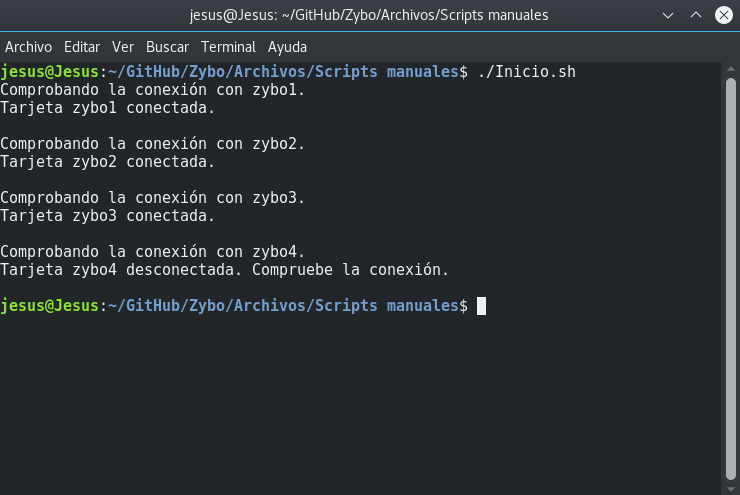
\includegraphics[scale=0.5]{Metodologia/Pruebas/Prueba_Inicio_sh.png}
	\caption{Prueba de \texttt{Inicio.sh}}
	\label{Prueba de Inicio.sh}
\end{figure}

\subsection{Software}
%\textcolor{red}{Prueba de funcionamiento de la recolección de datos: Una prueba de todo funcionando.}
Para realizar las pruebas de funcionamiento, basta con alimentar los nodos participantes en la cadena. En ese momento se ejecuta automáticamente los scripts descritos en el \hyperlink{Scripts}{Apéndice B}. 

Para el correcto funcionamiento de estos scripts, se requiere que el monitor central disponga del fichero inicial de datos creado por el usuario y que dicho usuario lo envíe al primer nodo de la red.

Hecho esto, sucede lo siguiente:
\begin{enumerate}
	\item Envío del fichero inicial a la primera tarjeta: Esto lo haremos gracias a la herramienta \texttt{sshpass} de Linux con la siguiente orden:
	\begin{center}
		\texttt{sshpass -p zyboX scp -o StrictHostKeyChecking=no archivoLocal zyboX@zyboX:/home/zyboX/ficheros/recibir}
	\end{center}
	Este proceso (Figura \ref{Fichero inicial en el ordenador central y envío al primer nodo}) lo podemos ver más detalladamente en el \hyperlink{EnvioRecepcionFicheros}{Apéndce A.4}.
	\begin{figure}[h]
		\centering
		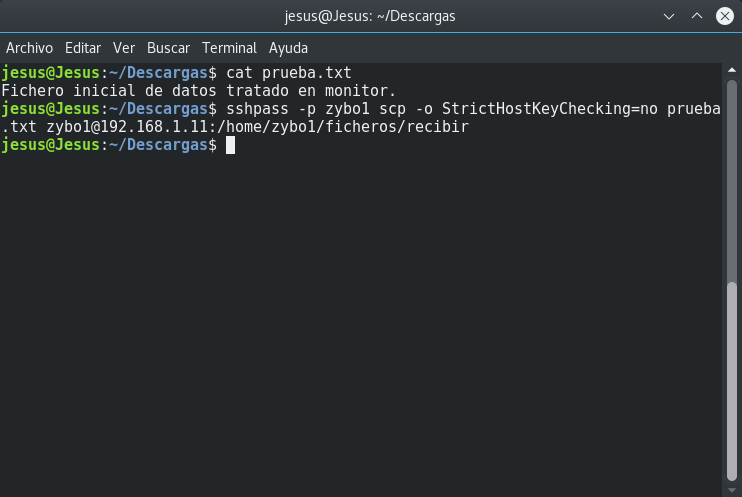
\includegraphics[scale=0.5]{Metodologia/Pruebas/Fichero_inicial_en_PC.png}
		\caption{Fichero inicial en el ordenador central y envío al primer nodo}
		\label{Fichero inicial en el ordenador central y envío al primer nodo}
	\end{figure}
\newpage
	\item Recepción del fichero en las tarjetas: Será el script \hyperlink{ScriptRecibiendo}{\texttt{Recibiendo.sh}} el encargado de comprobar la llegada del fichero y actuar en consecuencia cambiándolo de directorio.

	\item Modificación del fichero: El script \hyperlink{ScriptCristian}{\texttt{Cristian.sh}} será el encargado de abrir el fichero, modificarlo en cada una de las tarjetas y dejarlo preparado para su envío al siguiente nodo de la red. Para comprobar que los resultados de este script son correctos, podemos usar los comandos que vemos en la Figura \ref{Estado del fichero después de su modificación en Zybo1}.
	\begin{figure}[h]
		\centering
		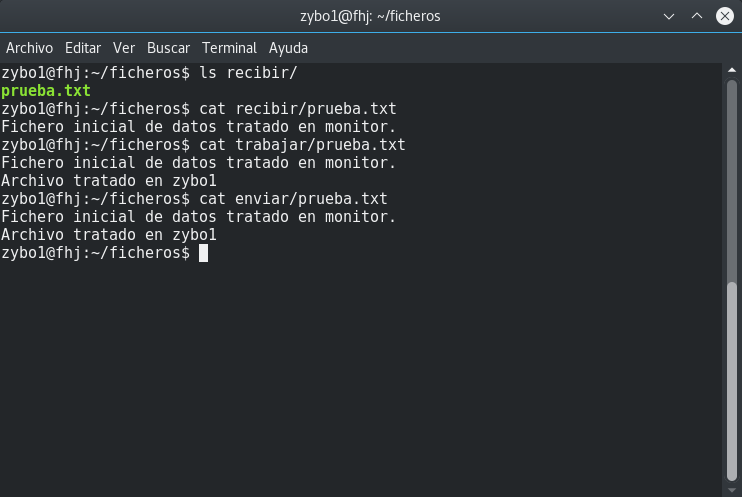
\includegraphics[scale=0.5]{Metodologia/Pruebas/Fichero_en_Zybo1.png}
		\caption{Estado del fichero después de su modificación en Zybo1}
		\label{Estado del fichero después de su modificación en Zybo1}
	\end{figure}
\newpage
	\item Envío del fichero hacia el siguiente nodo: Podemos distinguir dos tipos de envío del mismo fichero. Ambos llevados a cabo por el script \hyperlink{ScriptEnviando}{Enviando.sh}:
	\begin{enumerate}
		\item Tarjeta-Tarjeta: Esta opción se dará cuando la tarjeta actual detecte que la siguiente tarjeta está conectada.
		\item Tarjeta-Ordenador: Esta opción se dará cuando la tarjeta no detecte a la siguiente tarjeta. Entonces, enviará el fichero de datos, de vuelta al ordenador central.
	\end{enumerate}

\newpage
	\item Recepción del fichero en el ordenador central: El fichero final de datos, será recibido en el directorio\\ \texttt{/home/jesus/Vídeos} del ordenador central y contendrá los datos añadidos por todos los nodos de la red.
	\begin{figure}[h]
		\centering
		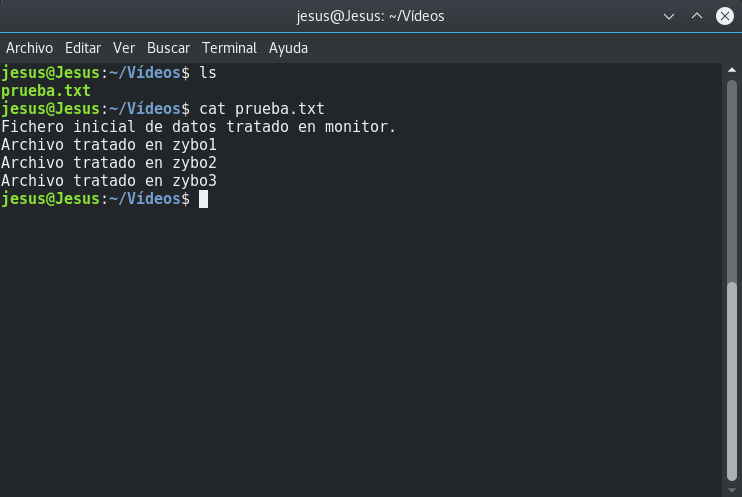
\includegraphics[scale=0.5]{Metodologia/Pruebas/Fichero_final_en_PC.png}
		\caption{Fichero final en el ordenador central}
		\label{Fichero final en el ordenador central}
	\end{figure}

\end{enumerate}

	\part{Eplílogo}
	\chapter{Manual de usuario}
\section{Introducción}
\textcolor{red}{Aquí poner lo que viene a ser los documentos míos, no?}

\section{Características}



\section{Requisitos previos}

	\chapter{Manual de instalación}
\section{Introducción}
\textcolor{red}{Alguna información adicional para hacer la instalación?}

\section{Requisitos previos}
\textcolor{red}{Tener disponibles los componentes necesarios(?)}

\section{Inventario de componentes}
\textcolor{red}{Enumeración de las tarjetas?}

\section{Procedimientos de instalación}
\textcolor{red}{Más manuales como el de mi documentación}

\section{Pruebas de implantación}
\textcolor{red}{Necesario?}
	\section{Conclusiones}
Después de las pruebas llevadas a cabo, podemos concluir el proyecto con un enfoque positivo. Gracias a la infraestructura de red creada, se ha conseguido con éxito una recopilación de datos colaborativa partiendo de un fichero inicial de datos desde el ordenador central, pasando por todos los nodos de la red y llegando, de nuevo, al ordenador central.

Además se ha conseguido que la información aportada por cada uno de los nodos de la red, está desligada de su dirección IP, de forma que, a priori, no se conozca la información que añadió cada nodo. El único inconveniente de esto es que, al ser una cadena secuencial, solo tendremos que saber qué nodos están conectados a la red para saber la información añadida por cada nodo.

Se pueden destacar varios escenarios de trabajo:
\begin{itemize}
	\item Si todos los nodos están conectados correctamente a la red, se producirá un recorrido lineal que partirá desde el ordenador central, viajará por todos los nodos desde zybo1 hasta zyboX. Una vez que se recorra toda la cadena y, al no detectar el siguiente nodo, zybo(X+1), el fichero retornará al ordenador central.
	\begin{figure}[h]
		\centering
		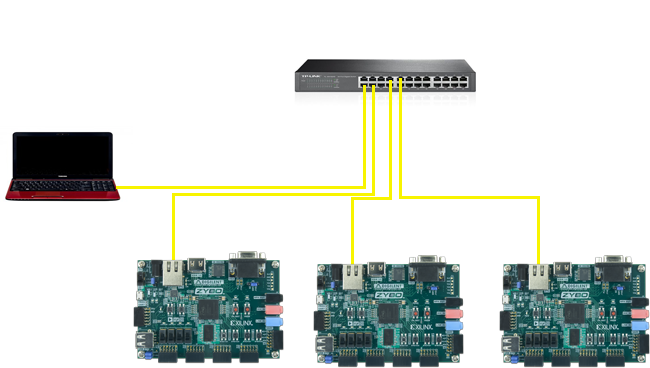
\includegraphics[scale=0.5]{Epilogo/RedCompleta.png}
		\caption{Red completa}
		\label{Red completa}
	\end{figure}
\newpage
	\item Cuando algún nodo intermedio de la red está desconectado, la cadena se romperá y, el nodo anterior, al no conseguir comunicación, enviará el fichero con la información recopilada al ordenador central, obviando el resto de nodos.
	\begin{figure}[h]
		\centering
		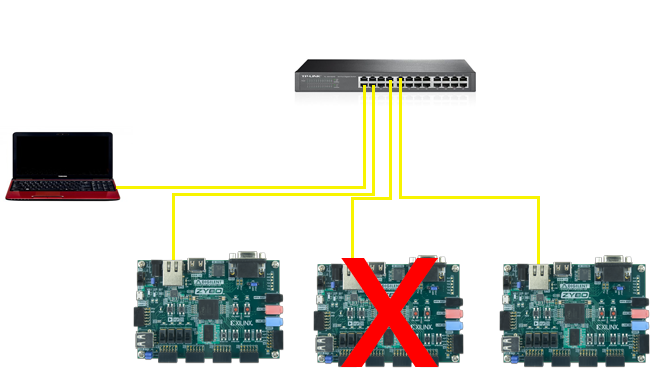
\includegraphics[scale=0.5]{Epilogo/RedSinNodo2.png}
		\caption{Red sin nodo intermedio}
		\label{Red sin nodo intermedio}
	\end{figure}
%\newpage
	\item Otro escenario será cuando el primer nodo de la red está desconectado.
	\begin{figure}[h]
		\centering
		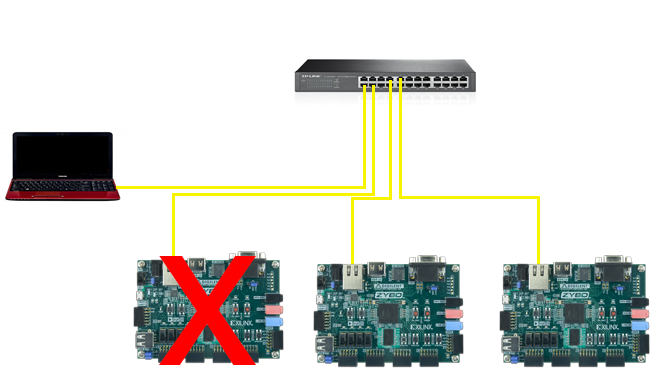
\includegraphics[scale=0.5]{Epilogo/RedSinNodo1.png}
		\caption{Red sin primer nodo}
		\label{Red sin primer nodo}
	\end{figure}\\
	Entonces, tendremos dos opciones:
	\begin{itemize}
		\item Volver a revisar la conexión con el primer nodo hasta conseguir solucionar el problema.
		\item Usar como primer nodo el segundo, enviando el fichero inicial directamente al segundo nodo de la red.
	\end{itemize}
\end{itemize}

Como ejemplo práctico de aplicación de esta red, se planteó como objetivo que la información aportada localmente por cada nodo fuera cifrada mediante un IP cifrador/descifrador AES \hyperlink{1}{[1]}. Para llevar a cabo esta aplicación, era necesario contar con el driver incluido en el sistema operativo compilado en otro Trabajo de Fin de Grado \hyperlink{2}{[2]}. A causa de la incompatibilidad de dicho sistema operativo compilado y los modelos de tarjeta Zybo utilizados en ambos proyectos, este objetivo no se ha podido completar.

\section{Trabajo futuro}
Como trabajo futuro quedaría cambiar la cadena de conexiones y que, en vez de recorrer los nodos de forma secuencial, se hiciera de forma aleatoria, para que no se supiera qué nodo ha seguido a cual. De esta forma, se conseguirá un desconocimiento total por parte del ordenador central sobre qué nodo añadió cada información al fichero final.

Para completar el trabajo de cifrado/descifrado de datos en la cadena de nodos de la red, deberíamos encontrar la compatibilidad con el sistema operativo aportado por el Trabajo de Fin de Grado de Gabriel Fernando Sánchez Reina. Una vez tengamos dicha compatibilidad y, debido a que dicho sistema operativo incluye el IP cifrador/descifrador de Cristian Ambrosio Costoya, ya podríamos realizar el cifrado/descifrado de los ficheros enviados por la red.

Otro posible uso de la red sería el tratamiento de una imagen, de modo que un IP dedicado a esto, formara parte del nodo de red.

También se podría mejorar el proyecto incluyendo un módulo Wi-Fi, de modo que los nodos, no tengan que estar necesariamente conectados por cable. Esto nos daría la posibilidad de ubicar cada nodo donde quisiéramos (dentro de las capacidades físicas de la red Wi-Fi) y así poder usar dicha estructura en un entorno de IoT\footnote{Internet of Things.} para una casa o el edificio que necesitemos. Para este cambio no haría falta modificar nada del software aportado por este proyecto.

	
%	%\textcolor{red}{Aquí empezaré a poner la bibliografía que constará de los foros y las páginas web que se han ido consultando a la hora de realizar el proyecto.}
%\begin{itemize}
\hspace{0.5cm}	[\hypertarget{1}{1}] IP cifrador/descifrador como Trabajo de Fin de Grado de Cristian Ambrosio Costoya. %Consultado el 20/02/2020.

\hspace{0.5cm}	[\hypertarget{2}{2}] Interfaz de conexión entre Linux y el IP cifrador/descifrador como Trabajo de Fin de Grado de Gabriel Fernando Sánchez Reina. %Consultado el 20/02/2020.

\hspace{0.5cm}	[\hypertarget{3}{3}] Manual de referencia oficial de DIGILENT: \url{https://reference.digilentinc.com/_media/zybo:zybo_rm.pdf}. Consultado el 15/05/2019.

\hspace{0.5cm}	[\hypertarget{4}{4}] Manual de SSH: \url{https://linux.die.net/man/1/ssh}. Consultado el 03/06/2019.

\hspace{0.5cm}	[\hypertarget{5}{5}] Manual de la herramienta \texttt{dd}: \url{https://man7.org/linux/man-pages/man1/dd.1.html}. Consultado el 20/08/2020.

\hspace{0.5cm}	[\hypertarget{6}{6}] Manual de la herramienta sshpass: \url{https://linux.die.net/man/1/sshpass}. Consultado el 10/06/2019.

\hspace{0.5cm}	[\hypertarget{7}{7}] Manual de scp: \url{https://linux.die.net/man/1/scp}. Consultado el 04/06/2019.

\hspace{0.5cm}	[\hypertarget{8}{8}] Compresión y descompresión de ficheros \url{http://ecapy.com/comprimir-y-descomprimir-tgz-} \url{tar-gz-y-zip-por-linea-de-comandos-en-linux/index.html}. Consultado el 20/05/2019.

\hspace{0.5cm}	[\hypertarget{9}{9}] Manual de stat: \url{https://linux.die.net/man/2/stat}. Consultado el 29/05/2019.

\hspace{0.5cm}	[\hypertarget{10}{10}] Manual de crontab: \url{https://linux.die.net/man/1/crontab}. Consultado el 03/06/2019.
	
\hspace{0.5cm}	[\hypertarget{11}{11}] Creación de diagramas de flujo gracias a la herramienta \url{https://app.diagrams.net/}. Consultado el 29/05/2019.
	
\hspace{0.5cm}	[\hypertarget{12}{12}] Clonación de tarjetas SD en Linux: \url{https://www.altaruru.com/como-clonar-una-sd-}\\
	\url{raspberry-pi-orange-pi/}. Consultado el 20/08/2020.

\hspace{0.5cm}	[\hypertarget{13}{13}] Protocolo SSH: \url{https://es.wikipedia.org/wiki/Secure_Shell} Consultado el 03/06/2019.
%\end{itemize}
	
\end{document}
